\documentclass[aspectratio=169]{beamer}
\usetheme{Madrid}
\usepackage{booktabs}
\usepackage{graphicx}
\usepackage{hyperref}

\title[Position-Restricted GemmaScope]{GemmaScope Position-Restricted Patch Checkpoint}
\subtitle{Model-merging SAE project}
\author{Local research checkpoint}
\date{2026-05-22}

\begin{document}

\begin{frame}
  \titlepage
  \begin{center}
    \small Checkpoint reason: position-restricted causal tests changed the mechanism claim.
  \end{center}
\end{frame}

\begin{frame}{Question}
  \begin{block}{What we tested}
    Use the same all-token top-delta GemmaScope MLP-SAE features, but restrict where they are patched during generation.
  \end{block}
  \begin{itemize}
    \item Positive control: patch all positions.
    \item Static prompt tests: content tokens, assistant boundary, prompt template, prompt all.
    \item Rollout tests: generated-token history, last token, prompt plus last token.
    \item Combined tests: assistant boundary plus generated history, content plus generated history, template plus generated history.
  \end{itemize}
\end{frame}

\begin{frame}{Main result}
  \begin{block}{Finding}
    The repair is not prompt-content semantics and not a static assistant-boundary-only patch.
  \end{block}
  \begin{itemize}
    \item `assistant boundary only' fails on the fully passing `12--20, 4:8' positive-control slice.
    \item `content only' and `content plus generated history' remain weak or zero.
    \item The best reduced mode is `assistant boundary plus generated history'.
    \item Mechanism hypothesis: restore an autoregressive refusal-state trajectory.
  \end{itemize}
\end{frame}

\begin{frame}{Heldout 4:8}
  \begin{center}
    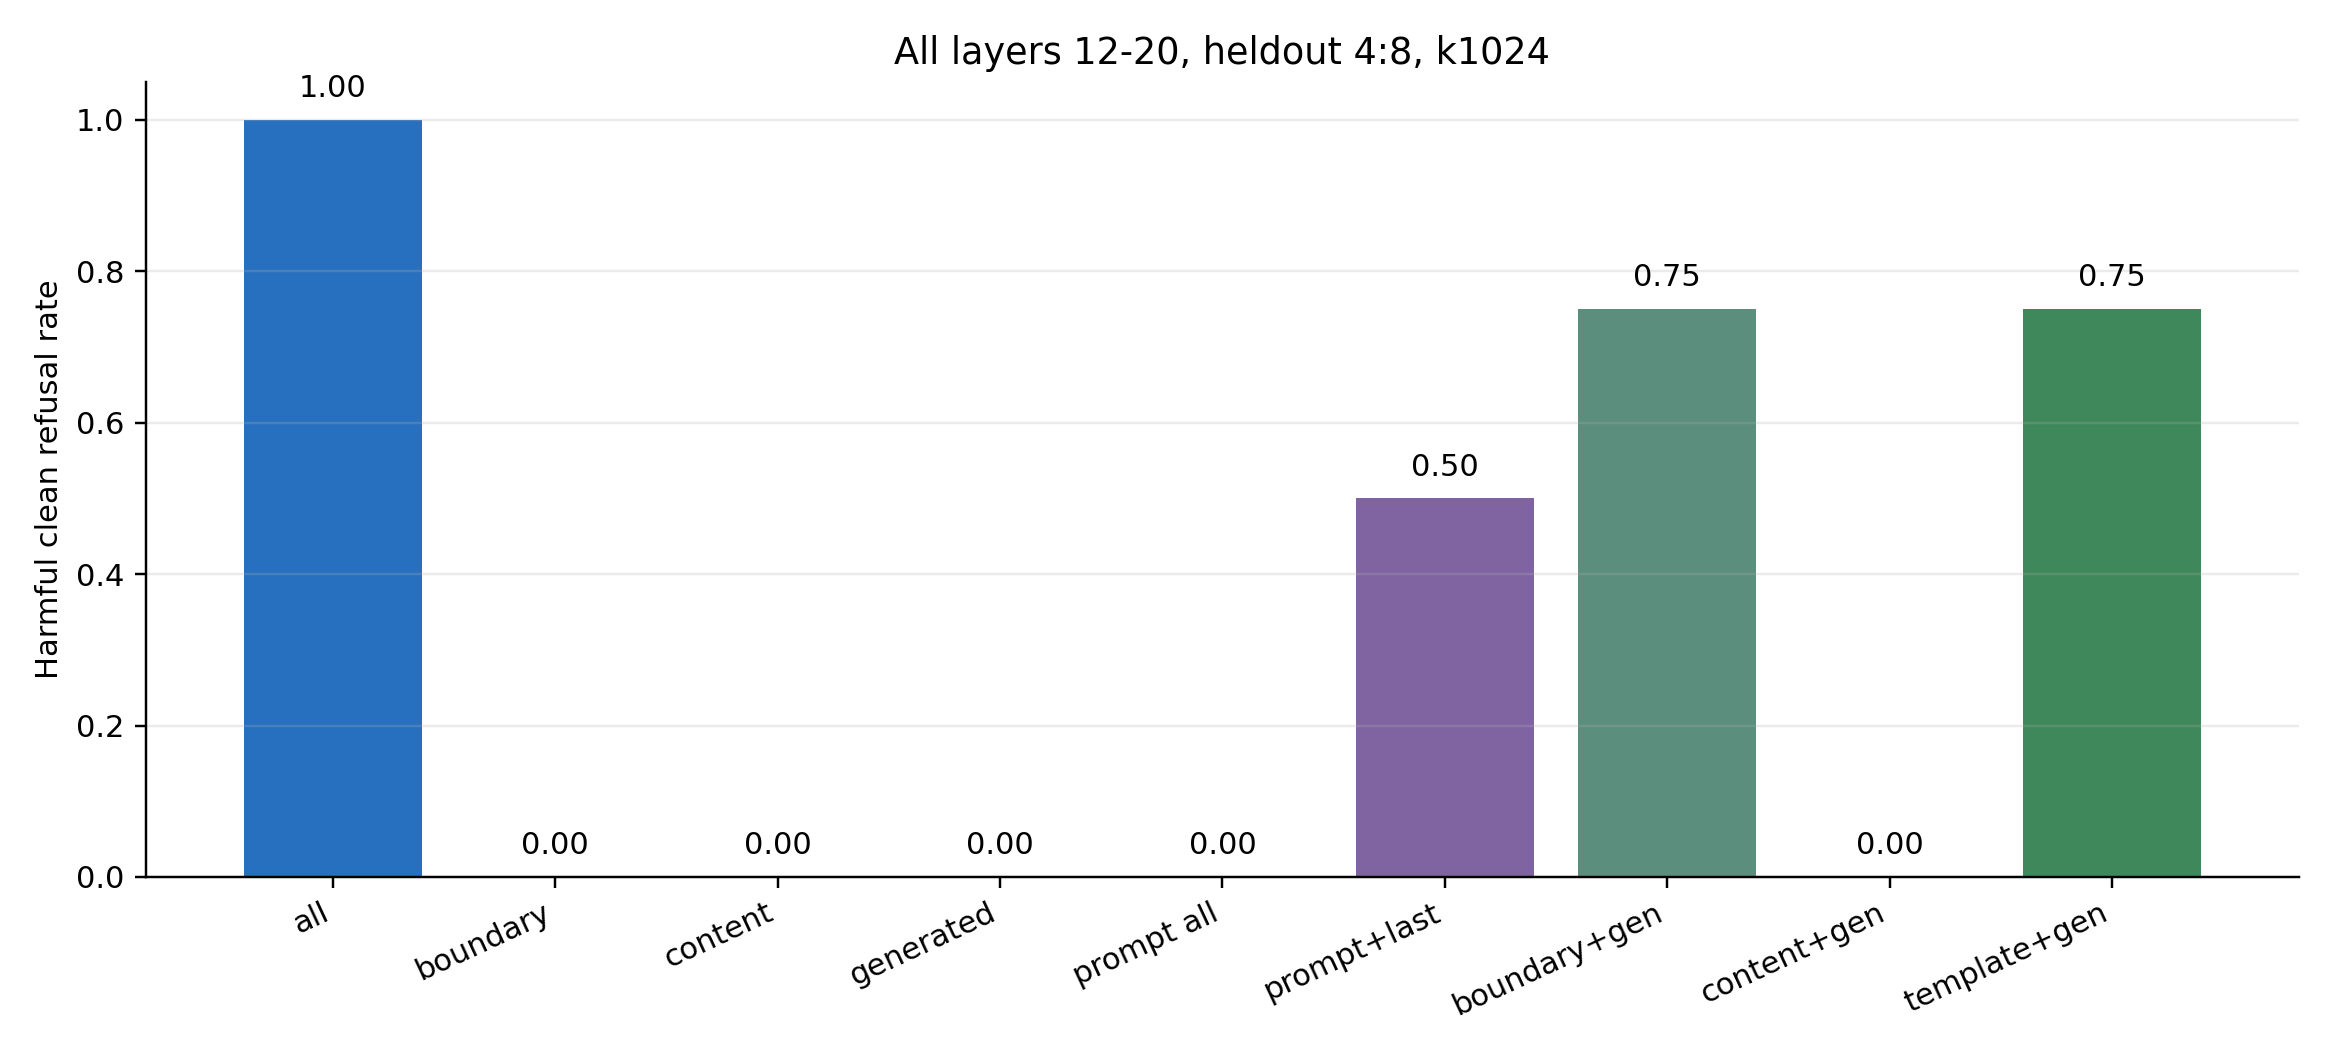
\includegraphics[width=0.94\linewidth]{figures/all_12_20_4_8_position_modes.png}
  \end{center}
  \vspace{-0.4em}
  \scriptsize All bars use layers 12--20, k1024 top-delta features. Y-axis is harmful clean refusal rate.
\end{frame}

\begin{frame}{Heldout 8:12}
  \begin{center}
    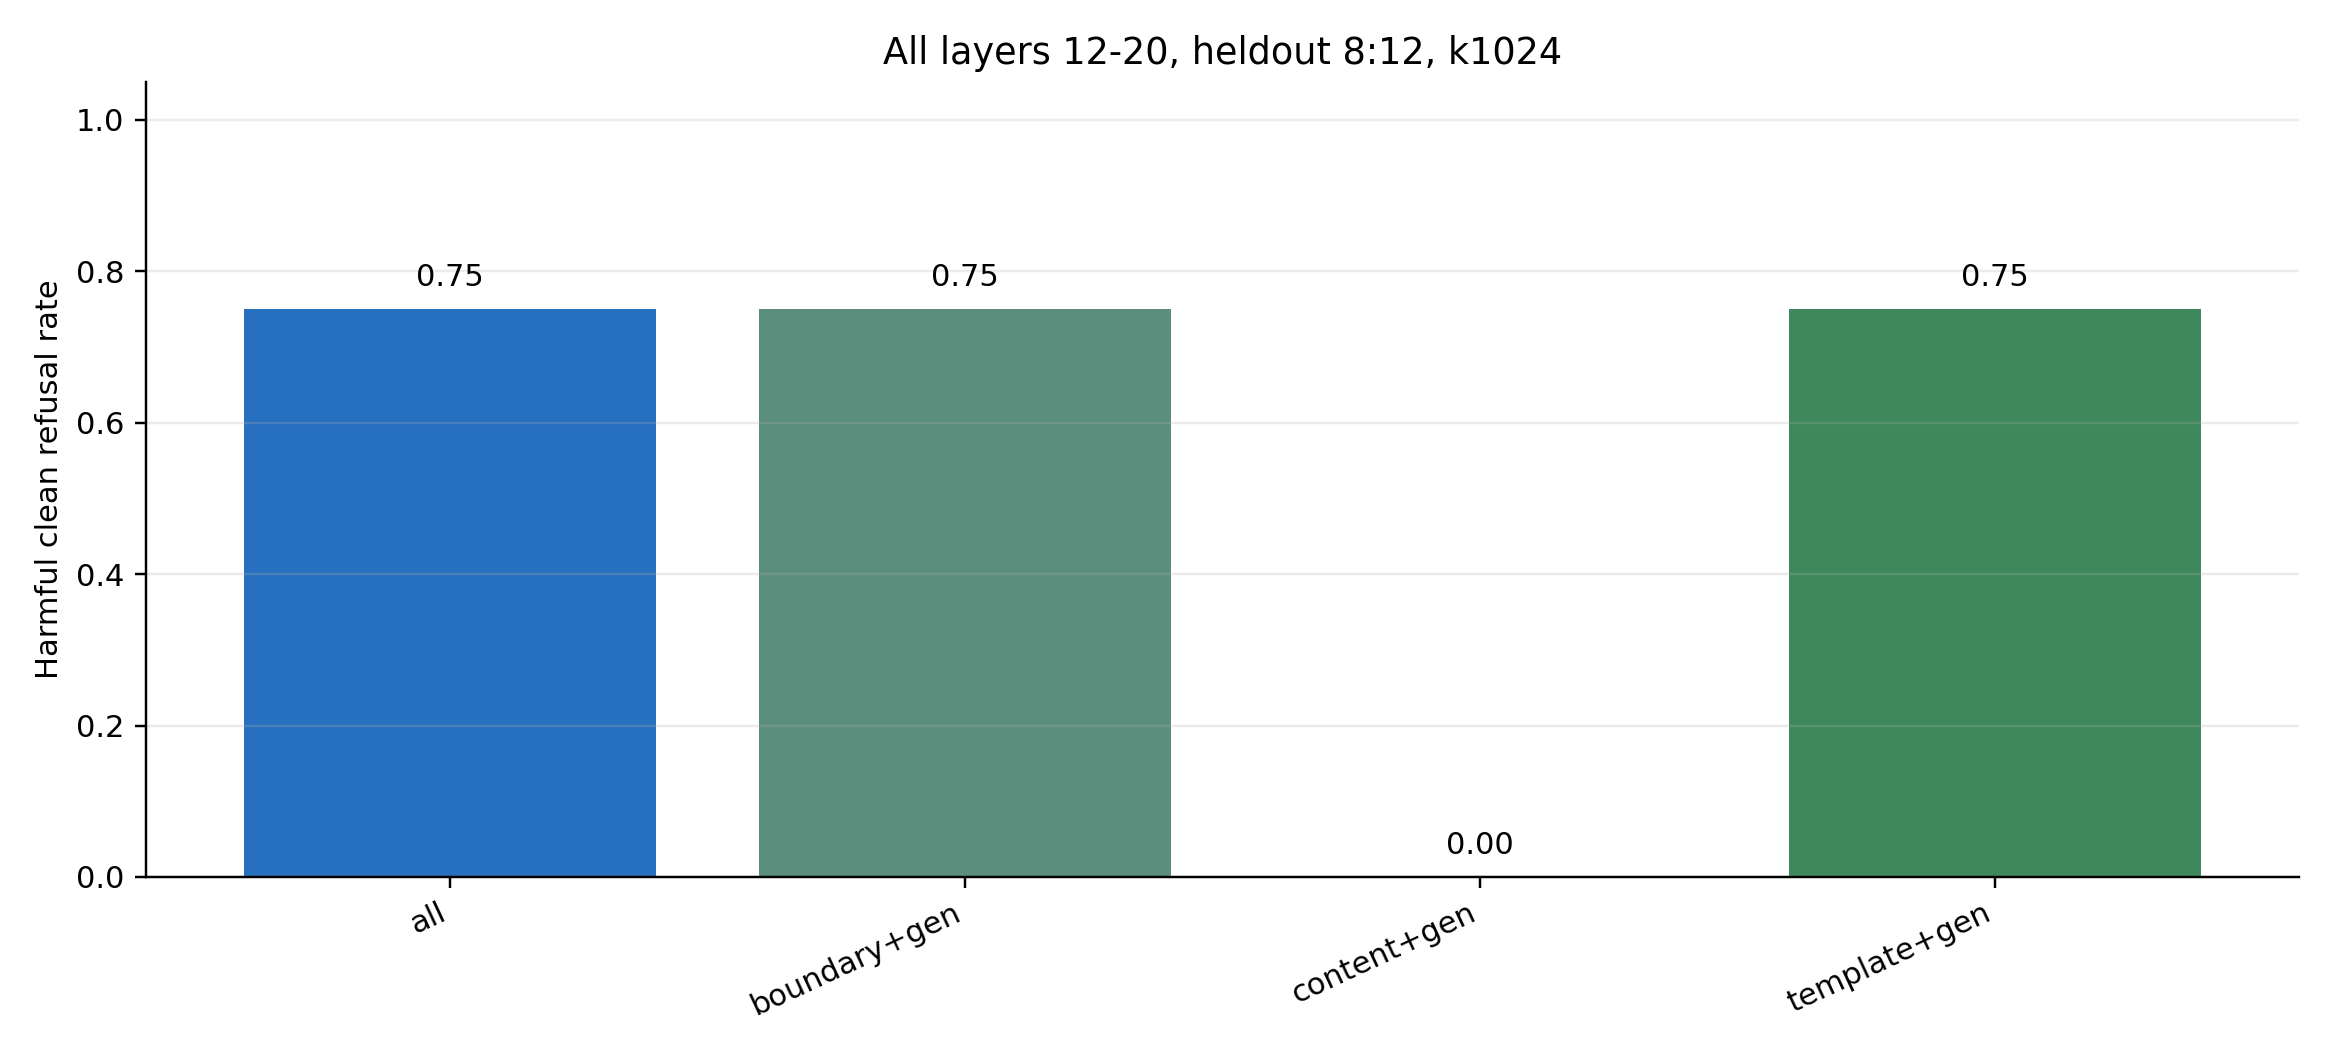
\includegraphics[width=0.94\linewidth]{figures/all_12_20_8_12_position_modes.png}
  \end{center}
  \vspace{-0.4em}
  \scriptsize Boundary+generated and template+generated match the all-position positive control on this fold.
\end{frame}

\begin{frame}{Key aggregate table}
  \scriptsize
  Cells are harmful clean refusal / unsafe continuation. Benign helpfulness is 1.000 for all rows shown.
  \vspace{0.5em}

  \begin{tabular}{llcccc}
    \toprule
    Layers & Slice & All & Boundary+gen & Content+gen & Template+gen \\
    \midrule
    12--20 & 4:8 & 1.000 / 0.000 & 0.750 / 0.000 & 0.000 / 0.000 & 0.750 / 0.000 \\
    12--20 & 8:12 & 0.750 / 0.000 & 0.750 / 0.000 & 0.000 / 0.000 & 0.750 / 0.000 \\
    15--20 & 4:8 & 1.000 / 0.000 & 0.750 / 0.250 & 0.250 / 0.000 & n/a \\
    15--20 & 8:12 & 0.500 / 0.500 & 0.500 / 0.250 & 0.000 / 0.250 & n/a \\
    \bottomrule
  \end{tabular}
\end{frame}

\begin{frame}{Interpretation}
  \begin{itemize}
    \item The boundary audit was directionally right, but incomplete: static boundary patching alone is not sufficient.
    \item Generated-token history is also not sufficient by itself.
    \item Repair needs a prompt-side template/boundary seed plus generated-history maintenance.
    \item For model merging, this suggests the missing object may be a response-state maintenance process rather than a standalone harmful-content feature.
  \end{itemize}
\end{frame}

\begin{frame}{Next tests}
  \begin{itemize}
    \item Repeat the reduced position modes at k2048.
    \item Identify which SAE feature IDs are necessary inside the boundary+generated condition.
    \item Time-slice generated-token history: early generated tokens only, late generated tokens only, or sustained patching.
    \item Then connect these causal features back to the merge/abliteration mechanism.
  \end{itemize}
\end{frame}

\begin{frame}{Local provenance}
  \scriptsize
  \begin{itemize}
    \item Summary: \texttt{\detokenize{data/GEMMA2_2B_GEMMASCOPE_MLP_SAE_POSITION_RESTRICTED_SUMMARY.md}}
    \item Metrics: \texttt{\detokenize{data/position_restricted_metrics.csv}}
    \item Source result root: \texttt{\detokenize{stage3/results/gemma2_2b_gemmascope_mlp_sae_position_restricted_atomic_v0/}}
    \item Main script: \texttt{\detokenize{stage3/scripts/run_gemma2_2b_gemmascope_mlp_sae_feature_subsets.py}}
    \item Aggregator: \texttt{\detokenize{stage3/scripts/aggregate_gemma2_2b_gemmascope_mlp_sae_position_restricted.py}}
  \end{itemize}
\end{frame}

\end{document}
